\documentclass{article}
\usepackage{amssymb, amsmath, amsthm}
\usepackage[margin=1in]{geometry}
\usepackage{verbatim}
\usepackage{graphicx}
\usepackage{hyperref} % \url \href
\usepackage{docmute}
\usepackage{blkarray}

\newtheorem{definition}{Definition}
\newtheorem{theorem}{Theorem}
\DeclareMathOperator{\spn}{Span}

\usepackage[style=chem-acs ,backend=bibtex, sorting=none]{biblatex}
\addbibresource{autoTB.bib}

\usepackage{tikz}

\usetikzlibrary{shapes.geometric, arrows}
\tikzstyle{startstop} = [rectangle, rounded corners, minimum width=2cm,text centered, draw=black]
\tikzstyle{process} = [rectangle, minimum width=2cm, text centered, draw=black]
\tikzstyle{decision} = [diamond, minimum width=2cm, text centered, draw=black]
\tikzstyle{arrow} = [thick,->,>=stealth]

\begin{document}

\section{METHODS}

In this section, we first describe the tight-binding method, which yield the physical 
properties of the materials in concern. We next show, on the other hand, that using results 
from group theory and symmetry, the free parameters in a tight-binding model can be 
greatly reduced. The higher crystal symmetry, the smaller number of free parameters are 
necessary to describe the electronic structure. This is the key result in this work.

\subsection{AO and Tight-binding Method}
Tight-binding methods is a well known technique to solve the band structure of 
crystalline material with a model Hamiltonian\cite{ziman_principles_1999}. 
It is fast to run and is able to reproduce the DFT calculated band structure accurately 
provided a suitable set of parameters. In this section, we provide a short review of the 
basic methods.

In the tight binding approximation, we write the Hamiltonian in some \emph{local}
basis orbitals:
\begin{equation}
    H_{\mu\nu}(R) = \langle \chi_{R',\mu} | H | \chi_{R'+R,\nu} \rangle = \langle \phi_{0,\mu} | H | \phi_{R,\nu} \rangle
\end{equation}
we use $|\chi_{R,\mu}\rangle$ to denote an electronic states on atom $\mu$ in the cell indexed by lattice vector $R$. 
Due to periodicity, we can arbitrarily choose $R'$ to be zero and arrive at the simplified expression.
The Bloch-like basis functions are given by:
\begin{equation}
    |\psi_{\nu}^k\rangle = \sum_R e^{ik\cdot(R+t_{\nu})} |\phi_{R\nu} \rangle
\end{equation}
and the Hamiltonian matrix at reciprocal vector $\mathbf{k}$ is related to the 
Hamiltonian in real space by:
\begin{equation}
    \label{E:TB}
    H_{\mu\nu}^{\mathbf{k}} = \langle \psi_{\mu}^k | H |\psi_{\nu}^k\rangle = \sum_R e^{ik\cdot(R+t_{\nu}-t_{\mu})} H_{\mu\nu}(R)
\end{equation}
Diagonalizing the square matrix $H_{\mu\nu}^{\mathbf{k}}$ gives the eigen energies $\varepsilon_{\mathbf{k}}$s 
at $\mathbf{k}$ in the tight-binding approximation. 

An important point in the tight-binding approximation is that the interaction matrix elements in real
space should decay rapidly, so that the number of $R$ in the summation \eqref{E:TB} can be greatly 
reduced. In the extreme case, nearest neighbor interactions are considered only. 
The decay depend on the spatial extension of orbitals $|\phi_{R,\nu}\rangle$. 
The valid of this approximate therefore depend on the chemical nature of the bonding. In this work, we use 
atomic orbitals (AOs) as basis functions and assume nearest neighbor interaction only to reduce the 
number of parameters in the model. 

Given set of tight binding parameters $H_{\mu\nu}(R)$, crystal Hamiltonian can be diagonalized at any $k$ points. Therefore, 
band structure and density of states can be obtained straightforwardly. We use tetrahedron method to solve for 
the density of states on a regularly spaced $\mathbf{k}$-grid. 

\subsection{Molecular Orbitals}
In this and following sections, we take a detour to visit the notion of symmetry adopted molecular orbitals. 
For the following, we label atomic orbitals using $|\chi_{\mu}\rangle$ and molecular orbitals $|\psi_i\rangle$. The $i^{th}$ molecular 
orbital can be expressed as a linear combination of atomic orbitals (LCAO): 
\begin{equation}
    \label{E:MO_equation}
    \psi_i\rangle = c_{i\mu} |\chi_{\mu}\rangle + \cdots + c_{i\nu} |\chi_{\nu}\rangle
\end{equation}
As will be described later, we form the linear combinations from a set of symmetry equivalent orbitals, i.e., orbitals 
on equivalent atoms, in a local scope. Therefore, this linear combination is finite and relatively small. For simplicity,
we assume that the atomic orbitals on different atoms have ignorable overlap, then the normalization 
of molecular orbital given by equation \eqref{E:MO_equation} is simply given by the normalization of the 
coefficients $\sum_{\mu}c_{i\mu}^2 = 1$.

The interaction energies in atomic orbitals and molecular orbitals are also related by the coefficients $c_{i\mu}$ as:
\begin{equation}
    \label{E:HAO_HMO_transformation}
    H_{ij} = \sum_{\mu} \sum_{\nu} c_{i\mu} c_{j\nu} H_{\mu\nu}
\end{equation}
where $H_{ij}$ and $H_{\mu\nu}$ are the interaction in terms of molecular orbitals and atomic orbitals. 

\subsection{Symmetry Adapted Molecular Orbitals}
For the moment, we focus on isolated moleculars and discuss the properties of symmetry adopted molecular 
orbitals (symmetry adopted linear combinations, SALCs). Later we discuss the application of similar treatment 
in the case of crystal by focusing on local fragments. 

The symmetry operations of a molecular form a group and symmetry groups provide a way to label different functions 
by its irreducible representations. We provide some more details in the appendix. The conclusion here is 
that the eigenfunctions of the Hamiltonian are also labelled according to the irreducible representations. Functions 
that belong to different irreducible representations have different symmetry properties and their Hamiltonian 
matrix elements will be zero unless the two wavefunctions belong to the same type of irreducible representations:
\begin{equation}
    \langle \psi_i^{\Gamma_a} | H | \psi_j^{\Gamma_b} \rangle = \delta_{ab}
\end{equation}
Furthermore, the energy will be degeneracy for two wavefunctions in the same irreducible:
\begin{equation}
    \langle \psi_1^{\Gamma_a} | H | \psi_1^{\Gamma_a} \rangle = \langle \psi_2^{\Gamma_a} | H | \psi_2^{\Gamma_a} \rangle
\end{equation}
These properties of functions labelled by irreducible representation that we utilize to find the minimum 
interaction parameters. 

In moleculars, we can find a suitable set of basis functions so that single electron states can be 
expressed as a linear combination of them. The set of basis functions form a vector space within which we 
can find SALCs that corresponding to certain irreducible representations. Using groups' character table, 
we can define a projection operator that project out a subspace of a given irreducible representation $\Gamma_i$:
\begin{equation}
    P^{\Gamma_i} = \frac{l_i}{h} \sum_R \chi^{\Gamma_i}(R) P_R
\end{equation}
where $R$ is a group operation, $P_R$ operate on the given functions. 
$l_i$ is the dimension of the representation, $h$ is the order of the group and
$\chi^{\Gamma_i}(R)$ is the character. To start with, we find a spanning basis for the vector space, which 
are simply each individual atomic orbtials we include. Applying the projection operator to each of these 
orbitals yields all wavefunctions that has the same symmetry properties.

We use group $D_{3h}$ and planar molecular AH$_3$ as an example. The 
three dimensional vector space span by three $s$ functions on each H atoms
is given by:
\begin{equation}
    V = \spn(|\chi^s_{1}\rangle, |\chi^s_2\rangle, |\chi^s_3\rangle)
\end{equation}
Using the projection operator, we find two subspaces corresponding to representation $A_1'$ 
and $E'$ with basis:
\begin{align}
    | \psi_1^{A_1'} \rangle &= \frac{\sqrt{3}}{3} (|\chi^s_1\rangle + |\chi^s_2\rangle + |\chi^s_3\rangle) \\
    |\psi_2^{E'}\rangle   &= \frac{\sqrt{6}}{6}( 2|\chi^s_1\rangle - |\chi^s_2\rangle - |\chi^s_3\rangle) \\
    |\psi_3^{E'}\rangle   &= \frac{\sqrt{6}}{6}(- |\chi^s_1\rangle + 2|\chi^s_2\rangle - |\chi^s_3\rangle)
\end{align}
We note that the two basis for representation $E'$ is not orthogonal.
To explore the most from symmetries, we can further split the representation $E'$ into one
that is symmetric and antisymmetric under mirror reflection, by descending symmetry $D_{3h}\to C_s$ (subduction):
\begin{align}
    |\psi_2^{E'_{D_{3h}}\to A'_{C_s}} \rangle &= \frac{2}{\sqrt{6}} |\chi^s_2\rangle - \frac{1}{\sqrt{6}} |\chi^s_1\rangle - \frac{1}{\sqrt{6}} |\chi^s_3\rangle \\
    |\psi_3^{E'_{D_{3h}}\to A''_{C_s}}\rangle &= \frac{\sqrt{2}}{2} |\chi^s_1\rangle - \frac{\sqrt{2}}{2} |\chi^s_3\rangle
\end{align}
The symmetrized molecular orbitals formed by the three $s$ functions are shown on the right panel of Figure \ref{F:AH3_MO}

\begin{figure}[h!]
    \centering
    \includegraphics{../figures/AH3_MO.pdf}
    \caption{Interactions allowed between $s$ and $p$ orbitals on atom A and $s$ functions on H atoms,
        belonging to a) representation $A_1'$, b) $E' \to A'$ (symmetric with respect to mirror reflection)
        and c) $E'\to A''$ (antisymmetric with respect to mirror reflection) }
    \label{F:AH3_MO}
\end{figure}

We follow the same method for sites in crystals. Interested in local interactions, we focus on one atomic site at a time and its neighbors. 
The symmetry group is therefore given by the site symmetry group of that atomic site. 
There are in total 32 possible site symmetry (point) groups in crystal and all of their character tables can be obtained from Bilbao. 
We can separate all atomic orbitals in a such a local cluster into different symmetry equivalent orbitals and obtain the basis functions 
for each irreducible representations. 
The method to identify site syemmtry and characters for each site symmetry operation are provided in the supplementary. 
To perform symmetry descend to separate degenerate subspaces, we choose the suitable subgroups that are able to separate degenerate 
subspace into representations of different symmetry properties, following the subduction tables 
given in \cite{altmann_point-group_1994}. In principle, the input atomic orbital vectorspace can be splitted into 
one dimensional subspaces. Although there can be multiple functions correspond to the same symmetry type, they belong to distinct 
subspaces and will not mix under symmetry operation. On the other hand, symmetry operation will mix subspaces that are separated 
by symmetry descend, for example, a three fold rotation will mix $|\psi_2^{E'_{D_{3h}}\to A'_{C_s}} \rangle$ with 
$|\psi_3^{E'_{D_{3h}}\to A''_{C_s}}\rangle$, which is the reason for their energy degeneracy.

\subsection{Interactions Between Symmetrized MOs}
In this section, we seek to systematically describe the form of $H_{ij}$, the interaction between molecular orbitals. We 
label the symmetry adopted MOs using notation
\begin{equation}
    \psi^{\Gamma_i^{(\alpha)} \to \Gamma_m}_A
\end{equation}
where the superscript denote the symmetry properties. $\Gamma_i$ is the representation symbol of the site symmetry group. 
In general, there can be multiple subspace that belong to the same representation and we use $(\alpha)$ to index them. 
$\Gamma_m$ is the symbol of irreducible representation of the subgroup. \emph{This superscript uniquely identify all molecular 
orbitals found from the previous section}. 
Subscript denote the set of symmetry equivalent orbitals from which this molecular orbitals come from, 
for example, $p$ orbitals on equivalent atoms $j$, which help to specify
the nature of the molecular orbtials. We have the following symmetry restrains for $H_{ij}$:
\begin{equation}
    \langle \psi^{\Gamma_i^{(\alpha)} \to \Gamma_m} |  H | \psi^{\Gamma_j^{(\beta)} \to \Gamma_n} \rangle 
    = 0 \quad \text{unless } \Gamma_i = \Gamma_j\text{ and } \Gamma_m = \Gamma_n
\end{equation}
i.e., interactions are only allowed between molecular orbtials with the same symmetry and 
\begin{equation}
    \langle \psi^{\Gamma_i^{(\alpha)} \to \Gamma_m} |  H | \psi^{\Gamma_i^{(\beta)} \to \Gamma_m} \rangle 
    = \langle \psi^{\Gamma_i^{(\alpha)} \to \Gamma_n} |  H | \psi^{\Gamma_i^{(\beta)} \to \Gamma_n} \rangle 
    = \cdots
\end{equation}
so that the value of the interactions are the same for corresponding molecular orbitals with the same symmetry 
under two subspaces. This allow us to write the matrix $H_{ij}$ in a block form, with blocks between two 
representations of the site symmetry group $\Gamma_i^{(\alpha)}$ and $\Gamma_j^{(\beta)}$, which is a 
diagonal matrix with identical diagonal value ($a\cdot \mathbf{I}$) if $\Gamma_i = \Gamma_j$, and all zero otherwise. 

In the example of AH3 molecular, the interaction between MOs on A atoms and MOs from H can be write as follows:
\begin{equation}
    H_{ij} = \begin{blockarray}{cccc}
        % & |s^{A_1'}\rangle & |p_z^{A_2''}\rangle & |p_x^{E'}\rangle & |p_y^{E'}\rangle 
        & \psi^{A_1'}_{H,s} & \psi^{E'\to A'}_{H,s} & \psi^{E'\to A''}_{H,s} \\
        \begin{block}{c(ccc)}
        \psi^{A_1'}_{A,s}      & a & 0 & 0 \\
        \psi^{A_2''}_{A,p}     & 0 & 0 & 0 \\
        \psi^{E'\to A'}_{A,p}  & 0 & b & 0 \\
        \psi^{E'\to A''}_{A,p} & 0 & 0 & b \\
        \end{block}
        \end{blockarray}
\end{equation}
The interactions are shown in Figure \ref{F:AH3_MO}. Graphically, it is not easy to see that 
$\langle \psi^{E'\to A'}_{A,p} | H | \psi^{E'\to A'}_{H,s} \rangle = \langle \psi^{E'\to A''}_{A,p} | H | \psi^{E'\to A''}_{H,s} \rangle$,
we derive this relationship in the Appendix.


\subsection{Eliminating symmetry equivalent interactions}
We want to identify the minimum set of interations $H_{\mu\nu}$ which allow the generation of the entire tight-binding Hamiltonian, and we show 
here that the relationship between different $H_{\mu\nu}$s are encoded by $H_{ij}$. This procedure simplifies the size of 
the parameter finding problem as well as ensure the correct symmetry of the Hamiltonian. In the context of machine learning, recent advance in 
rotational invariant models automatically gives some relationship between different $H_{\mu\nu}$s, however, as illustrated by 
the following example, using representation theory, all symmetry relationship can be discovered in a systematic way. 

\begin{figure}[h!]
    \centering
    \includegraphics{../figures/S-Px.pdf}
    \caption{Interaction between $p_x^l \leftrightarrow s \leftrightarrow p_x^r$ on a linear molecular. 
                a) Interactions is not allowed by symmetry, and b) Interaction is allowed}
    \label{F:s_px_chain}
\end{figure}

We consider the simple case of $p_x^l \leftrightarrow s \leftrightarrow p_x^r$ interaction as shown in Figure \ref{F:s_px_chain}, 
where superscript $l$ and $r$ indicate left and right, in 
a site symmetry of $C_s$ (mirror). Suppose the interaction $s$--$p_x^r$ is $a$, it is apparent to us that the interaction $p_x^l$--$s$ is $-a$. However,
fact is not apparent for an rotational invariant machine learning model, because it is not possible to transform $p_x^l$
into $p_x^r$. 
On the second hand, due to symmetry, the two $p_x$ function can be combined into a symmetric and anti-symmetric part, and 
only the symmetric part interact with the $s$ function. So we have:
\begin{align}
    \label{E:px_s_AO_MO}
    \langle s | H | \psi_A'' \rangle = \frac{\sqrt{2}}{2} \left( \langle s | H | p_x^l \rangle + \langle s | H | p_x^r \rangle\right) = 0 \\
    \langle s | H | \psi_A' \rangle = \frac{\sqrt{2}}{2} \left( \langle s | H | p_x^l \rangle - \langle s | H | p_x^r \rangle\right) = b
\end{align}
which readily give the solution  $\langle s | H | p_x^l \rangle = \langle s | H | p_x^r \rangle = b/2$. 

When parameter $b$ is not known, we will have one equation only, in which case the value of $\langle s | H | p_x^l \rangle$ and 
$\langle s | H | p_x^r \rangle$ can not be solved. However, from the first equation, it is clear that only one of the two 
is free parameter. In more complicated case, free parameters can also be found in this way, since we can find a set of linear equations
\begin{gather}
    \sum_{\mu} \sum_{\nu} c_{1\mu} c_{2\nu} H_{\mu\nu} = H_{12} \\
    \sum_{\mu} \sum_{\nu} c_{1\mu} c_{3\nu} H_{\mu\nu} = H_{13} \\
    \cdots \\
    \sum_{\mu} \sum_{\nu} c_{i\mu} c_{j\nu} H_{\mu\nu} = H_{ij} 
\end{gather}
where many rows are zero on the right side, we can establish a homogeneous equation with number of rows $m$ less than number of 
unknown $n$. In such case, we will have in general $m-n$ free variables. To find these variable, we transform the 
coefficient matrix $C_{m\times n}$ into a row echelon form and each column without a leading variables would correspond to 
a free parameters. In this work, we use Gaussian elimination to bring the coefficient matrix to row echelon form.

\subsection{Generation of Tight-binding Hamiltonian}
Once suitable values are assigned to each of the free variables, values of all the unknowns can be found by appending to the homogeneous 
equation with rows, each has the free variables on the left and their corresponding on the right. This procedure produce a full rank 
coefficient and an linear equation system with unique solution. 

\begin{figure}[h!]
    \centering
    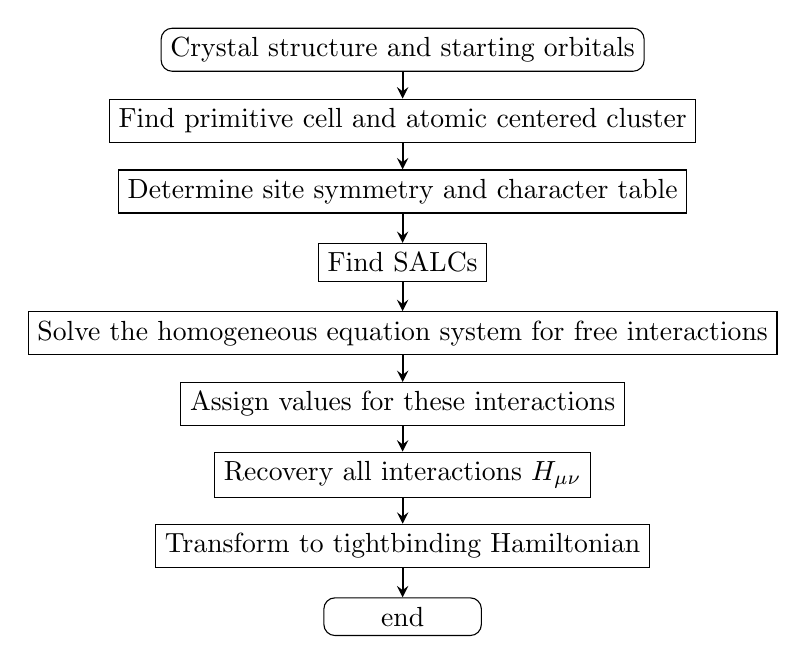
\begin{tikzpicture}[node distance=0.9cm]
        \node (start) [startstop] {Crystal structure and starting orbitals};
        \node (pro1) [process, below of=start] {Find primitive cell and atomic centered cluster};
        \draw [arrow] (start) -- (pro1);
        \node (pro2) [process, below of=pro1] {Determine site symmetry and character table};
        \draw [arrow] (pro1) -- (pro2);
        \node (pro3) [process, below of=pro2] {Find SALCs};
        \draw [arrow] (pro2) -- (pro3);
        \node (pro4) [process, below of=pro3] {Solve the homogeneous equation system for free interactions};
        \draw [arrow] (pro3) -- (pro4);
        \node (pro5) [process, below of=pro4] {Assign values for these interactions};
        \draw [arrow] (pro4) -- (pro5);
        \node (pro6) [process, below of=pro5] {Recovery all interactions $H_{\mu\nu}$};
        \draw [arrow] (pro5) -- (pro6);
        \node (pro7) [process, below of=pro6] {Transform to tightbinding Hamiltonian};
        \draw [arrow] (pro6) -- (pro7);
        \node (end) [startstop, below of=pro7] {end};
        \draw [arrow] (pro7) -- (end);
    \end{tikzpicture}
    \caption{Workflow of the generation of Tightbinding Hamiltonian}
    \label{F:workflow_Hamiltonian}
\end{figure}

To bring everything together, the workflow to generate the tight-binding Hamiltonian 
is organized as Figure \ref{F:workflow_Hamiltonian}. We start by finding atomic centered 
clusters and the vector space formed by the choosen starting basis. After finding 
site symmetry operations, we assign symmetry group and characters of each operations in the 
irreducible representations. The character table, together with subduction relationship, 
enable us to obtain the symmetry adopted molecular orbitals. The constrains 
given by symmetry allow us to reduce the number of free atomic interactions to the minimum 
number possible. Until this moment, there are no concrete values involved in the process.
Then, provided the values for each free atomic interactions, we are able to solve 
for all values of the interactions which we need for the formulation of tightbinding Hamiltonian.
After Hamiltonian in reciprocal space is obtained, electronic structure and derived properties 
can be extracted by solving the eigen values for the Hamiltonian. 

Our implementation is written in Python with numpy and are fully modulized. We provide solver 
for bandstructure with interface to Seekpath library for high symmetry k-path. Density of states
can be solved using tetrahedron summation method, provided with the code. We also offer 
interface to BoltzTrap2 for the solution of transport properties through linearized Boltzmann 
transport equations.

\end{document}
